\documentclass{beamer}
\usetheme{Boadilla}
\usepackage{graphicx}
\graphicspath{ {~/Documents/plsc31101-final-project/Code/} }

\setlength{\parskip}{1em}


\title{Introduction to LaTeX}
\author{Livia Dewaele}

\begin{document}

\begin{frame}
\titlepage
\end{frame}

\begin{frame}
\frametitle{What is LaTeX?}
\begin{itemize}
	\setlength\itemsep{1em}
	\item A method of creating documents using plain text. It is stylized using markup tags, a bit like HTML. \\
	\item Not a word processor: you don't change the style manually, like in Word. \\
	\item As you type, you mark the document structure with tags eg title. \\
	\item Everything is compiled into a final document at the end.
\end{itemize}
\end{frame}

\begin{frame}
\frametitle{Why use LaTeX?}
\begin{itemize}
	\setlength\itemsep{1em}
	\item Stylistic uniformity.
	\item Sophisticated structuring abilities.
	\item Reference tracking.
	\item Use different set templates, eg to make articles, books, reports, letters, presentations, etc.
	\item Very good for printing mathematical equations etc, figures, tables...
\end{itemize}
\end{frame}

\begin{frame}
\frametitle{First Steps}
\begin{itemize}
	\setlength\itemsep{1em}
	\item In order to use LaTeX, you need to install a LaTeX editor. It is free and open source. 
	\item Once you have downloaded it, open TexStudio and you are ready to go.
\end{itemize}
\end{frame}


\begin{frame}
\frametitle{Document structure}
\begin{itemize}
	\setlength\itemsep{1em}
	\item	Like in R, there are commands and comments in LaTeX. Commands start with a backslash and comments start with percentage sign. 
	\item Here is an example of how you would begin making a LaTeX document:
\end{itemize}
\end{frame}

\begin{frame}[fragile]
\frametitle{Including Code}
\begin{semiverbatim}
\\documentclass[a4paper,12pt]{article}
\\begin{article}
A sentence of text.
\\end{article}
\end{semiverbatim}

\begin{itemize}
	\setlength\itemsep{1em}
	\item 'documentclass': at the beginning of every Latex document, you need to specify which Latex template you are going to use.
	\item 'begin' and 'end': commands that enclose the text and commands that make up the doc.
	\item Anything before 'begin' (known as the preamble) or after 'end' is not printed.
\end{itemize}
\end{frame}


\begin{frame}[fragile]
\frametitle{Creating a document}
\begin{itemize}	
	\setlength\itemsep{1em}
	\item You can customize your LaTeX doc by using packages:
	 	\begin{itemize}	
	 	\item These are put in the preamble. 
		\item The command is:
		\begin{semiverbatim}
		 \\usepackage{name}
		 \end{semiverbatim}
		 \end{itemize}
	\item You can create a title by filling in the title in the preamble, like this:
	\begin{semiverbatim}
	 \\title{ My Title Here}
	  \end{semiverbatim}
	  \item To print the title in the document, use the maketitle command within the document (after 'begin'):
	  \begin{semiverbatim}
	   \\maketitle 
	    \end{semiverbatim}
	\item To create an output, press the 'Typeset' button in the corner (like 'knit' in R).
\end{itemize}
\end{frame}


\begin{frame}
\frametitle{How does it look?}
Here is an example of what some 'complete' LaTeX document (in this case for this presentation) would look like:
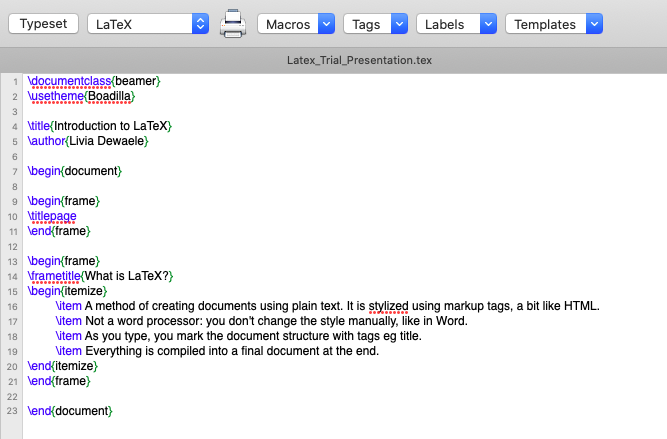
\includegraphics[scale=0.4]{lateximage.png}



\end{frame}


\begin{frame}
\frametitle{More Information about LaTeX}

I created a full document taking you through the main functions of LaTeX - please see this if you are interested in learning more!

Otherwise there are some other great resources. Here are two useful links: 

LATEX for Beginners Workbook Edition 5.
\hyperlink{LATEX for Beginners Workbook Edition 5} {http://www.docs.is.ed.ac.uk/skills/documents/3722/3722-2014.pdf}

Wikibooks Introduction to LaTeX.
\hyperlink{Wikibooks Introduction to LaTeX} {https://en.wikibooks.org/wiki/LaTeX/Introduction}

\end{frame}
	
	
	
	
	
	
\end{document}